%======================================================================
\chapter{Tutorials}
%======================================================================

%----------------------------------------------------------------------
\section{USB Connection}
%----------------------------------------------------------------------
\begin{enumerate}
    \item Verify QuaRC is installed on computer
    \item Install QFLEX 2 USB into Quanser Aero as seen in Figure~\ref{fig:USB_Panel}
    \item Open Simulink model
    \item Connect Quanser Aero to computer via the included USB adapter cable
    \item Set simulation mode to external
    \item Run MATLAB initialization code for motion controller
    \item Click "Build Model" button
    \item Click "Connect To Target" button
    \item Click "Run" button
\end{enumerate}

\begin{figure}[!h]
    \centering
    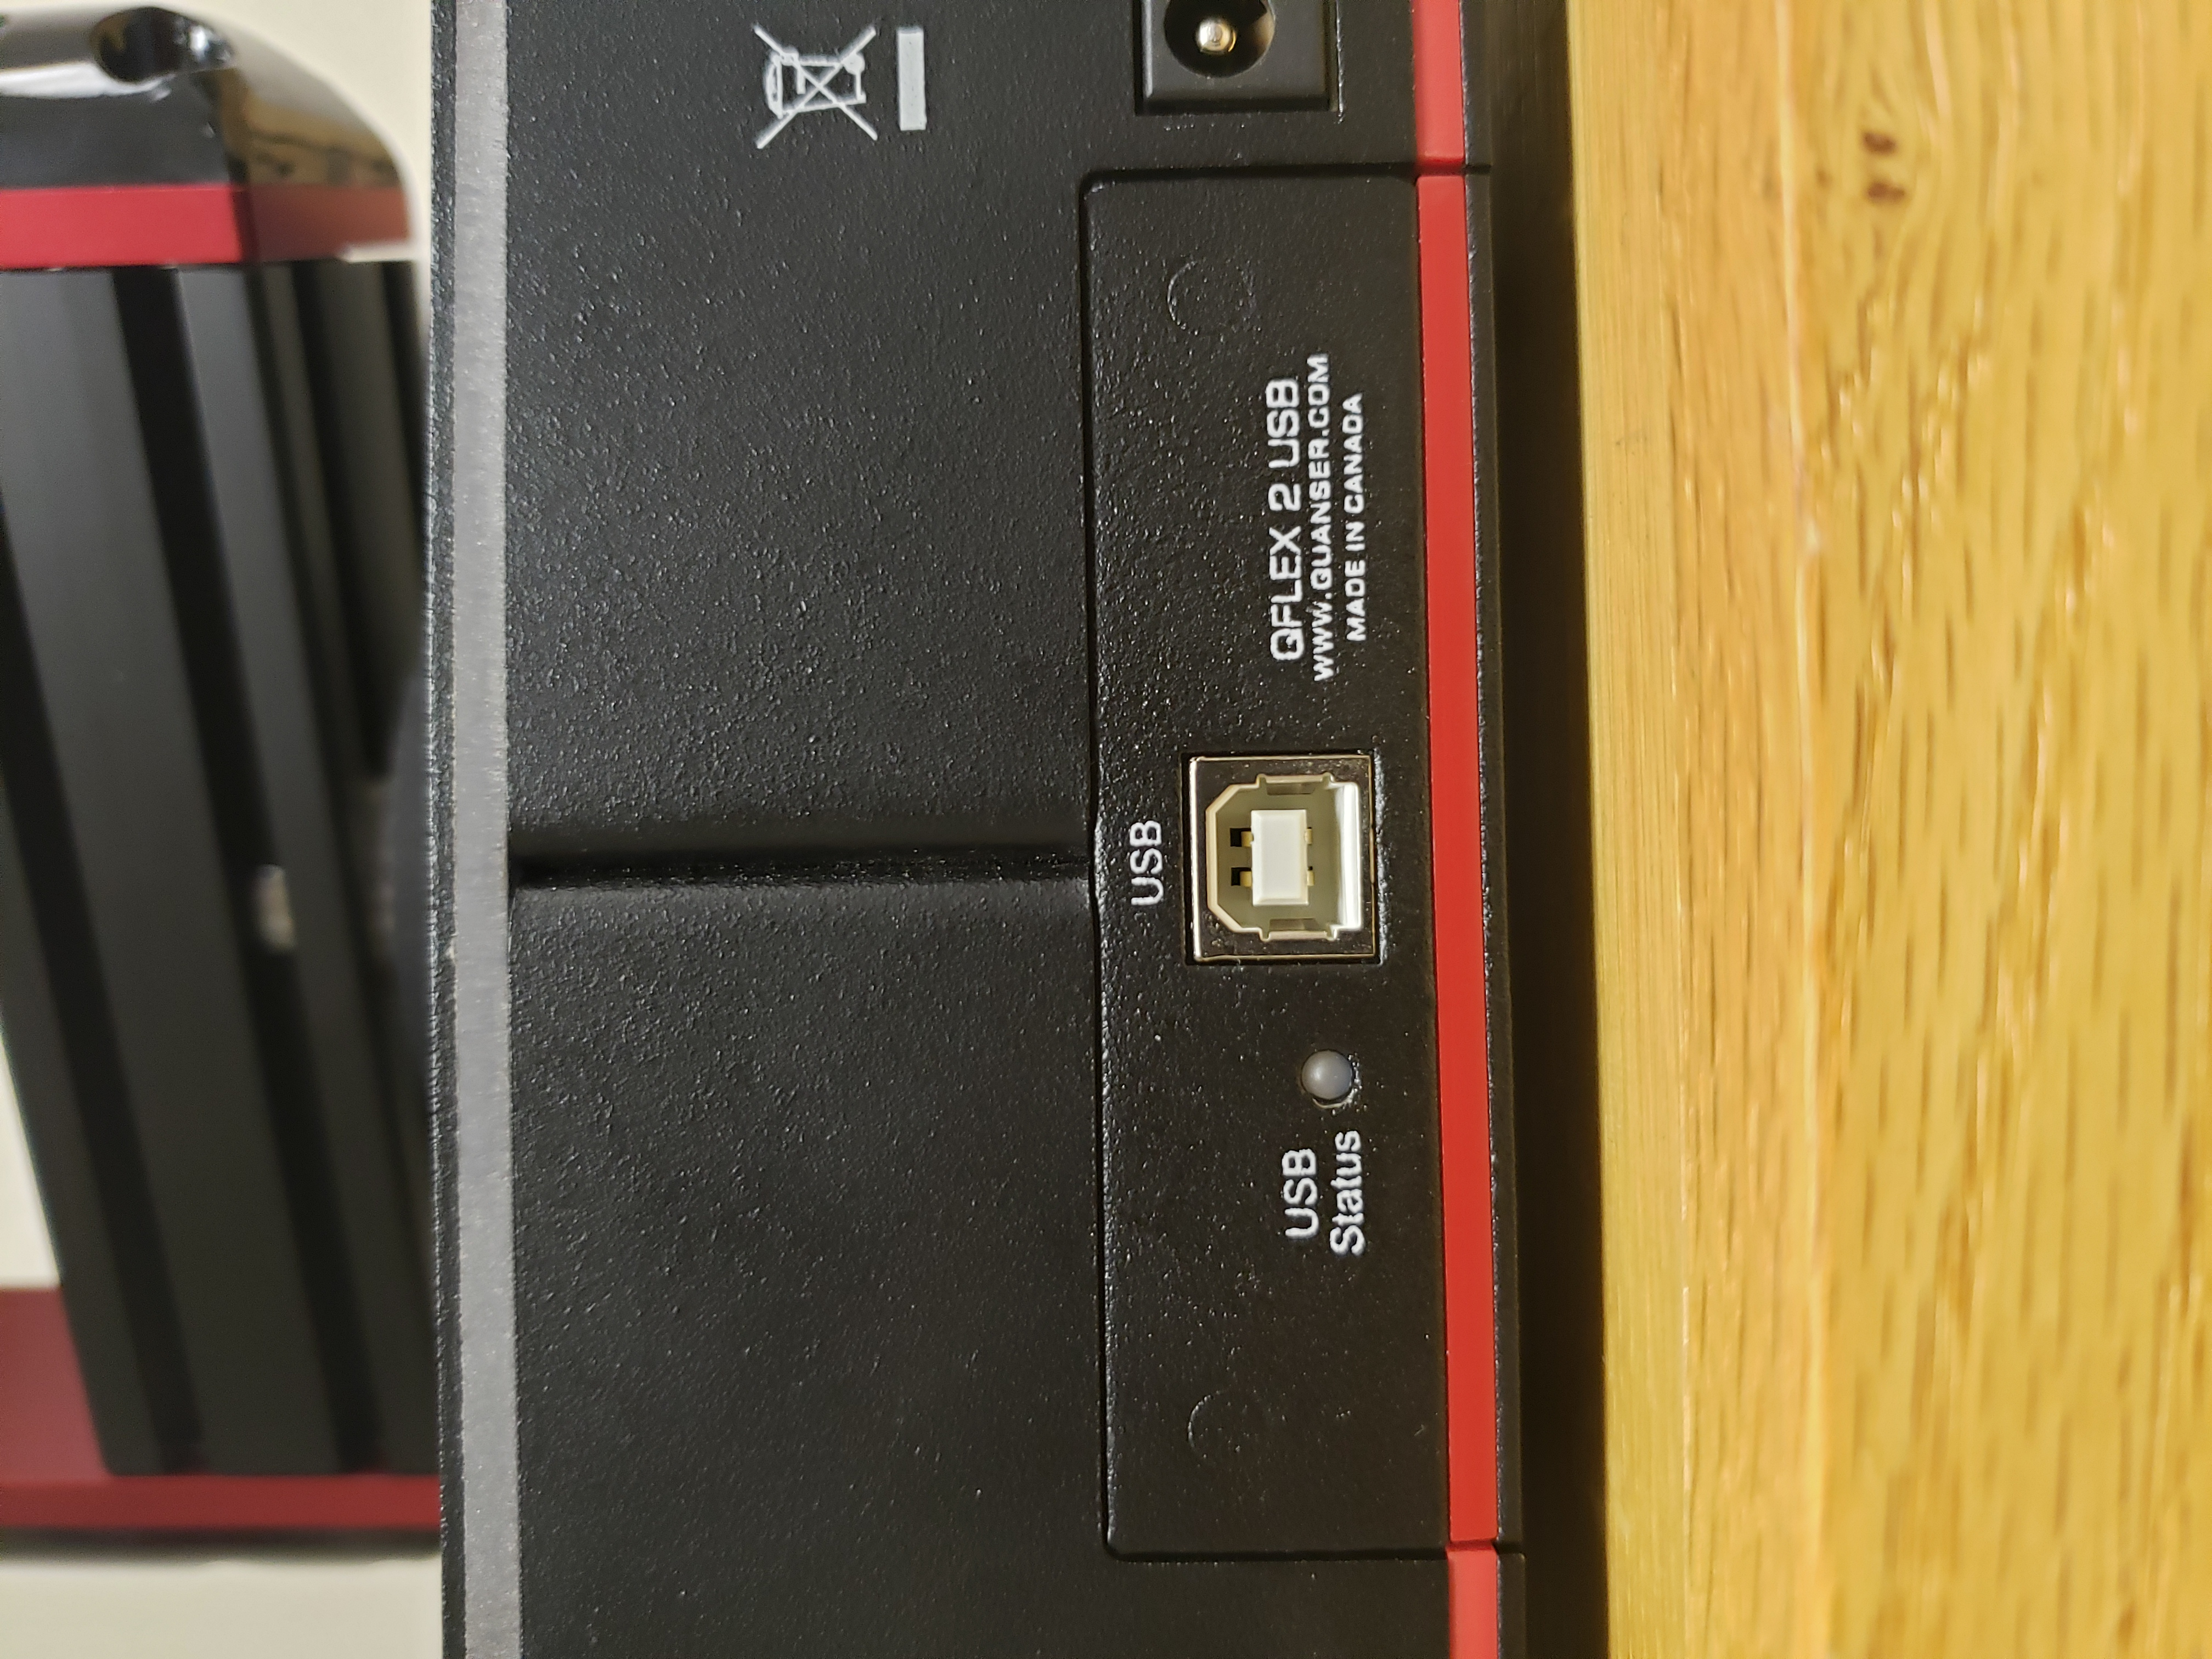
\includegraphics[angle = 270,width=.248\textwidth,keepaspectratio=true]{figs/img/USB_Panel.jpg}
    \label{fig:USB_Panel}
    \caption{Quanser Aero with QFLEX 2 USB panel installed}
\end{figure}
%----------------------------------------------------------------------
\section{Raspberry Pi Implementation}
%----------------------------------------------------------------------
\begin{enumerate}
    \item Make sure software add ons are installed on MATLAB
    \begin{enumerate}
        \item MATLAB Support Package for Raspberry Pi Hardware
        \item Simulink Support Package for Raspberry Pi Hardware
    \end{enumerate}
    \item Install QFLEX 2 Embedded into Quanser Aero as seen in Figure~\ref{fig:Embedded_Panel}
    \item Assuming Raspberry PI is not connected to network, establish a serial connection to the Raspberry PI
    \item \todo[inline]{Setup Raspberry PI on the network}
    \item Connect SPI wires to Raspberry PI. Pin 1 (white wire) on the embedded panel connects to +5V on the Pi.  Pin 2 (yellow wire) connects to GPIO 10 on the Pi. Pin 3 (blue wire) connects to GPIO 9 on the Pi.  Pin 4 (green wire) connects to GPIO 11 on the Pi. Pin 6 (purple wire) connects to GPIO 8 on the Pi.  Pin 7 (Red wire) connects to ground on the Pi.
    \item Connect Raspberry PI to QFLEX 2 Embedded
    \item Right click on Simulink model
    \item Open "Model Configuration Parameters"
    \item Select "Hardware Implementation"
    \item Set "Hardware Board" to "Raspberry Pi"
    \item Under "Board Parameters" under "Groups" type in the IP address of the Raspberry PI, the username, and password
    \item Under "Build options", set build action to "Build and run" and type in the file path that you want the model to be stored on the Raspberry PI
    \item Set simulation mode to external
    \item Run MATLAB initialization code for motion controller
    \item Run MATLAB Raspberry PI/SPI initialization code \ref{ch:RPI3_SPI_Int}
    \item Click "Deploy to Hardware" button
    \item To stop program you must "kill" it
    \item Open Putty, connect to your Raspberry PI, and log in
    \item Type "ps -A" to view running programs and find the process number of your Simulink model
    \item Type "sudo kill -9 \#\#\#\#" where \#\#\#\# is your process number.  This will kill the program
\end{enumerate}

\begin{figure}[!h]
    \centering
    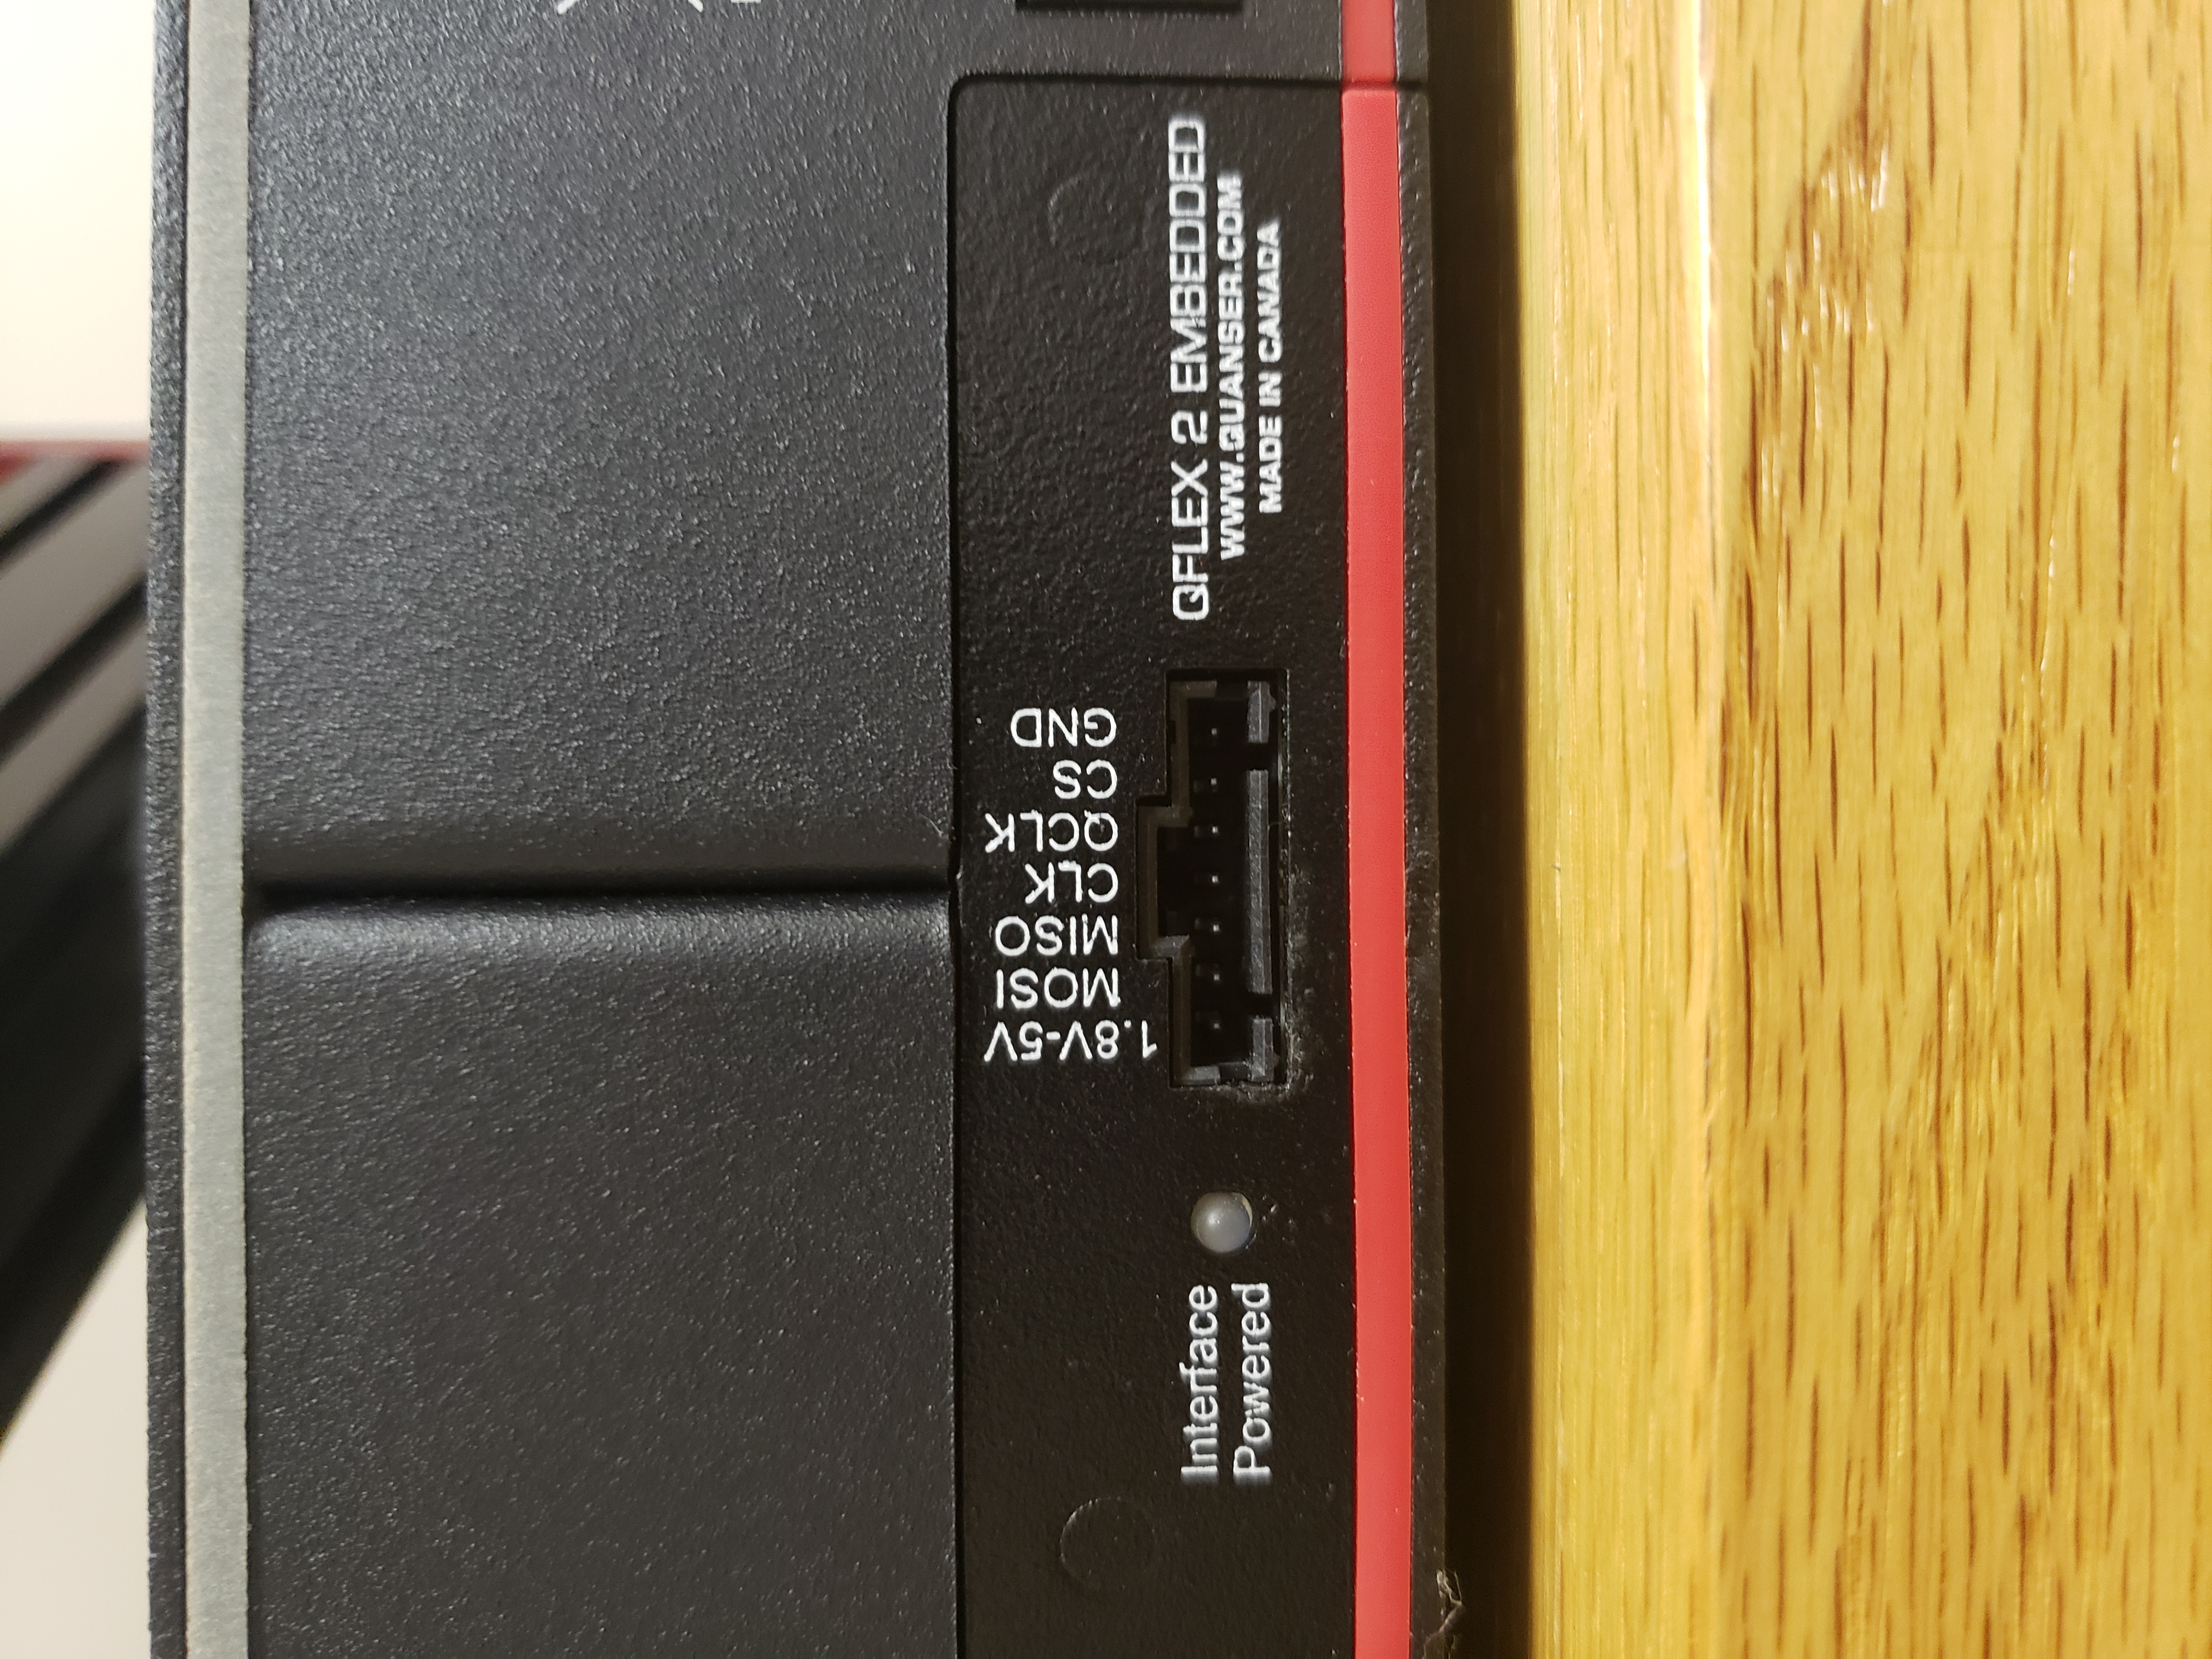
\includegraphics[angle = 270,width=.248\textwidth,keepaspectratio=true]{figs/img/Embedded_Panel.jpg}
    \label{fig:Embedded_Panel}
    \caption{Quanser Aero with QFLEX 2 Embedded panel installed}
\end{figure}
%----------------------------------------------------------------------
\section{Android Application}
%----------------------------------------------------------------------


%%% Local Variables:
%%% mode: latex
%%% TeX-master: "../finalReport"
%%% End:
